\section{Entanglement}
    \hypertarget{defentro1}{}
    \begin{tcolorbox}[vert]
        Let be 2 parts: $A & B, \mathspace \mathcal{H}_{\text{total}}=\mathcal{H}_A \otimes \mathcal{H}_B$, then there is two types of states: 
        \begin{align*} 
            \text{\textbf{product states: }} &\ket{ \psi}=\ket{\phi_A}\otimes\ket{\chi_B}, \\
            \text{\textbf{entangled states: }} &\ket{\psi} \text{ such that } \nexists \text{ a factorization into tensor product. }
        \end{align*}
    \end{tcolorbox}
    \begin{remark}{Example}
        \begin{tcolorbox}[rouge]
            Let $\mathcal{H}_{\text{total}}=\mathbb{C}^2 \otimes \mathbb{C}^2, \mathspace \ket{\psi}=\alpha_{00}\ket{00}+\alpha_{01}\ket{01}+\alpha_{10}\ket{10}+\alpha_{11}\ket{11}, \mathspace \ket{ab}=\ket{a}\otimes\ket{b}, \mathspace a_{ij}\in\mathbb{C}, \mathspace\sum_{ i,j=\left(0,0\right) } ^{ \left(1,1\right) }\left|\alpha_{ij}\right|^2=1, \mathspace \braket{\psi|\psi}=1$.
            \textbf{Product state:} 
            
            \vspace{5pt}
            $\ket{\psi}=\left(\alpha\ket{0}+\beta\ket{1}\right)\otimes\left(\gamma\ket{0}+\delta\ket{1}\right)  $
            such that $\alpha_{00}=\alpha \gamma, \alpha_{01}= \alpha \delta, \alpha_{10}=\beta \gamma, \alpha_{11}= \beta \delta$.

            \vspace{5pt}
            det$\begin{pmatrix} \alpha_{00} & \alpha_{01} \\ \alpha_{10} & \alpha_{11} \end{pmatrix} = det\left(\alpha\right)_{ij}=\alpha_{00}\alpha_{11}-\alpha_{01}\alpha_{10}=\alpha \gamma \beta \delt=- \alpha \delta \beta \gamm=0$.

             $\ket{\psi}$ \important{ is a product state } $\iff$ det$\begin{pmatrix} \alpha_{00} & \alpha_{01} \\ \alpha_{10} & \alpha_{11} \end{pmatrix}=0$.
              \end{tcolorbox}
        
    \end{remark}     
    \begin{remark}{}
        \begin{tcolorbox}[rouge]
            \textbf{Entangled state: }


            We will use the Bell states: 
            \begin{itemize}[left=10pt, label=\textbullet]
                \item $\ket{B_{00}}=\frac{1}{\sqrt{2}}\left(\ket{00}+\ket{11}\right)$
                \item $\ket{B_{01}}=\frac{1}{\sqrt{2}}\left(\ket{01}+\ket{10}\right)$
                \item $\ket{B_{10}}=\frac{1}{\sqrt{2}}\left(\ket{00}-\ket{11}\right)$
                \item $\ket{B_{11}}=\frac{1}{\sqrt{2}}\left(\ket{01}-\ket{10}\right)$
            \end{itemize}
            Properties:
            \begin{enumerate}[left=10pt]
                \item They form an orthonormal basis of $\mathbb{C}^2 \otimes \mathbb{C}^2$
                \[\braket{B_{ij}|B_{ij}}=1, \mathspace \braket{B_{ij}|B_{kl}}, \mathspace \left(ij\right)\neq\left(kl\right).\]
                \item ``Rotation invariance'': $\ket{B_{00}}=\frac{1}{\sqrt{2}}\left(\ket{\theta}\otimes \ket{\theta}+\ket{\theta_{\perp}}\otimes \ket{\theta_{\perp}}\right) \forall \theta$.
            \end{enumerate}
        \end{tcolorbox}
    \end{remark}
    \subsection{Teleportation}
        \begin{tcolorbox}[vert]
            The goal of teleportation is to teleport a quantum state or some information from A to B without physically transporting any qubit, we will however send classical messages
        \end{tcolorbox}
        \begin{itemize}[left=10pt, label=\textbullet]
            \item \textbf{Initial situation: } 
            \[\overbrace{\mathbb{C}_1^2 \otimes \mathbb{C}_2^2}^{Alice} \otimes \overbrace{\mathbb{C}_3^2}^{Bob}, \mathspace \ket{\phi}_1=\alpha \ket{0}_1 + \beta \ket{1}_1, \mathspace \ket{B_{00}}_{23}=\frac{1}{\sqrt{2}}\left(\ket{00}+\ket{11}\right).\]
            
        \begin{center}
        \begin{tikzpicture}[scale=1.2, every node/.style={font=\small}]
            \node[circle, fill=black, inner sep=2pt, label=left:{$1$}] (A1) at (0,0) {};
            \node[circle, fill=black, inner sep=2pt, label=left:{$2$}] (A2) at (0,0.8) {};
            \node at (0, 1.5) {A};
            \node[circle, fill=black, inner sep=2pt, label=right:{$3$}] (B3) at (3,0.8) {};
            \node at (3, 1.5) {B};
            \node at (1.6, 1.25) {entangled pair $\ket{B_{00}}_{23}$}
            \draw[thin] (1.5,0.8) ellipse [x radius=1.65, y radius=0.3];
        \end{tikzpicture}
        \end{center}
        \item \textbf{Final situation: }
        \[\ket{B_{??}}_{12},\mathspace\ket{\phi}_3=\alpha \ket{0}_2+\beta\ket{1}_3.\]
        \begin{center}
        \begin{tikzpicture}[scale=1.2, every node/.style={font=\small}]
            \node[circle, fill=black, inner sep=2pt, label=left:{$1$}] (A1) at (0,0) {};
            \node[circle, fill=black, inner sep=2pt, label=left:{$2$}] (A2) at (0,0.8) {};
            \node at (0, 1.5) {A};
            \node[circle, fill=black, inner sep=2pt, label=right:{$3$}] (B3) at (3,0.8) {};
            \node at (3, 1.5) {B};
            \node at (1.6, 0.4) {entangled pair $\ket{B_{??}}_{23}$}
            \draw[thin] (0,0.4) ellipse [x radius=0.2, y radius=0.6];
        \end{tikzpicture}
        \end{center}
        \item \textbf{Protocol steps:}
                \begin{enumerate}[left=10pt]
                    \item Alice does a Bell basis measurement in her lab, so her qubits collapse into one of the fourth possible Bell states, the total state becomes 
                    \[\left(\ket{B_{ij}}_{12}\bra{B_{ij}}_{12} \otimes \mathbbm{1}_3\right)\ket{\phi}_1 \otimes \ket{B_{00}}_{23}=\ket{B_{ij}}_{12} \otimes \ket{\widetilde{\phi}}_3.\]
                    \item Alice sends two classical bits of information to Bob: 00, 01, 10, 11.
                    \item Bob receives a classical message $ij \in \{00, 01, 10, 11\}$ and does the following: 
                    \begin{align*} 
                        00 &\to \text{Bob applies } \mathbbm{1} \text{ on his qubit}, \\
                        01 &\to \text{Bob applies } X_3 = \begin{pmatrix} 0 & 1 \\ 1 & 0 \end{pmatrix} \text{ on his qubit}, \\
                        10 &\to \text{Bob applies } Z_3 = \begin{pmatrix} 1 & 0 \\ 0 & -1 \end{pmatrix} \text{ on his qubit}, \\
                        11 &\to \text{Bob applies } Z_3X_3 = \begin{pmatrix} 0 & 1 \\ -1 & 0 \end{pmatrix} \text{ on his qubit}, \\
                    \end{align*}
                \end{enumerate}
        \end{itemize}
    \subsection{Dense coding}
        \begin{tcolorbox}[vert]
            The goal is to send two classical bits from A to B of information by one use of quantum channel.
        \end{tcolorbox}
        \begin{center}
        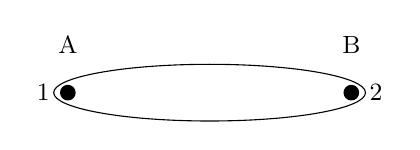
\begin{tikzpicture}[scale=1.2, every node/.style={font=\small}]
            \node[circle, fill=black, inner sep=2pt, label=left:{$1$}] (A1) at (0,0) {};
            \node at (0, 0.5) {A};
            \node[circle, fill=black, inner sep=2pt, label=right:{$2$}] (B2) at (3,0) {};
            \node at (3, 0.5) {B};
            \draw[thin] (1.5,0) ellipse [x radius=1.65, y radius=0.3];
        \end{tikzpicture}
        \end{center}
        \textbf{Protocol:}

            If Alice wants to encode 
            \begin{align*} 
                00 &\to \text{she applies } \mathbbm{1}_1 \otimes \mathbbm{1}_2 \ket{B_{00}}_{12}=\ket{B_{00}}_{12}, \\
                01 &\to \text{she applies } X_1 \otimes \mathbbm{1}_2 \ket{B_{00}}_{12}=\ket{B_{01}}_{12}, \\
                10 &\to \text{she applies } Z_1 \otimes \mathbbm{1}_2 \ket{B_{00}}_{12}=\ket{B_{10}}_{12}, \\
                11 &\to \text{she applies } Z_1X_1 \otimes \mathbbm{1}_2 \ket{B_{00}}_{12}=\ket{B_{11}}_{12}, \\
            \end{align*}
            Then she sends her obtained qubit so Bob have both qubit $\to$ the total state. So he knows which bits Alice encoded.

